\documentclass[11pt,twocolumn]{amsart}

\usepackage{amsmath}
\usepackage{physics}
\usepackage[margin=0.2in]{geometry}
\usepackage{graphicx}
\usepackage{listings}

\setcounter{section}{-1} 

\begin{document}
\section{Physical constants}
$k=1.381\times10^{-23}J/K = 8.617\times10^{-5}eV/K$, $N_A = 6.022\times10^{23}$, $R=8.315 J/mol\cdot K$, $h=6.626\times10^{-34}J\cdot s = 4.136\times10^{-15}eV\cdot S$

\section{Energy in Thermal Physics}

\subsection{Thermal equilibrium}
\emph{Temperature} is a measure of the tendency of an object to spontaneously give up energy to its surroundings. When two objects are in thermal contact, the one that tends to spontaneously \emph{lose} energy is at the \emph{higher} energy. Room temperature $~300K$

\subsection{The ideal gas} $PV = nRT = Nk_BT$. $n$ is no of moles, $N=nN_A$ is number of molecules. $k_B = R/N_A$. Latter equation is valid when avg. space b/w molecules is larger than size of molecules. $\bar{E}_{K,trans} = \frac{3}{2}kT$.

\subsection{Equipartition of energy}
Theorem: at temperature $T$, the average energy of any quadratic degree of freedom is $\frac{1}{2}kT$. $U_{thermal} = Nf\frac{1}{2}kT$. Monoatomic gas: $f=3$. Diatomic gas: $f=5,6$ (3 trans., 2-3, rot.) or $f=8$ (3 trans., 3 rot., 2 vibr. K, P). Solid: $f=6$ (6 vibr. 3K, 3P). Some vibrational energies may be "frozen out" at room temperature.

\subsection{Heat and work}  
First law of thermodynamics \\$\Delta U = Q + W$. The change in energy is equal to the heat added and the work done. Heat transfer happens by \emph{conduction}, \emph{convection} and \emph{radiation}.

\subsection{Compression work}
Consider a piston. The force is $F=PA$. Assumes that the pressure is uniform. Compression must be slow enough so the gas has time to continually equilibrate to the changing conditions $\rightarrow$ \emph{quasistatic}. A compressed gas, i.e. negative $\Delta V$ gives $W=F\Delta x=PA\Delta x = -P\Delta V$. 
\subsubsection{Compression of ideal gas}
Two idealised ways: \\ \emph{Isothermal} compression is so slow that the temperature of the gas does not rise (quasistatic). \emph{Adiabatic} compression is so fast that no heat escapes during the compression. $VT^{f/2}=\text{constant}$, $V^{\gamma}P=\text{constant}$. $\gamma=\frac{f+2}{f}$ is the adiabatic exponent.

\subsection{Heat capacities}
Amount of heat needed to raise an object's temperature, per degree temperature increase: $C = \frac{Q}{\Delta T} = \frac{\Delta U - W}{\Delta T} $. $W=0$ and $V =\text{constant}$ is called heat capacity heat capacity at \emph{constant volume}, else there would be compression work, $-P\Delta V$. $C_V=\left(\frac{\partial U}{\partial T}\right)_V$. If an object expand when heated and do work on surroundings, there is negative $W$. At constant $P$, $Q$ i unambiguous $\rightarrow$ heat capacity at \emph{constant pressure}: $C_P = \left(\frac{\Delta U -(-P\Delta V)}{\Delta T}\right)_P=\left(\frac{\partial U}{\partial T}\right)_P + P\frac{\partial V}{\partial T}_P$.
\subsubsection{Latent heat} During a phase transformation \\ $C = \frac{Q}{\Delta T} = \frac{Q}{0} = \infty$. While $L=\frac{Q}{m}$ is the heat required to accomplish the transformation, the \emph{latent heat}.
\subsubsection{Enthalpy} To create a rabbit out of nothing, the sorcerer must summon up not only the energy $U$ of the rabbit, but also some additional energy, equal to $PV$, to push the atmosphere out of the way to make room. The \emph{enthalpy}: $H= U + PV$. At constant $P$, $\Delta H = Q + W_{other}$.

\section{The Second Law}
Entropy, and multiplicity, tends to increase.
\subsection{Two-state systems} 
Multiplicity is given by the binomial coefficient. $\Omega(N,n) = \frac{N!}{n!\cdot (N-n)! } = \binom{N}{n}$. How many ways to pick $n$ objects out of $N$. Permutations: $_nP_k = n(n-1)(n-2)\dots (n-k) = \frac{n!}{(n-k)!} $. Unordered permutations: $_nC_k = _nP_k / k! = \binom{n}{k}$. This is the binomial coefficient. Binomial distribution: $\binom{n}{k}p^k(1-p)^{(n-k)}$.
\subsection{Einstein model of a solid} 
One energy unit is $h\nu = \hbar\omega$. Multiplicity of Einstein solid with $N$ oscillators (N/3 atoms) and $q$ energy units: $\Omega(N,q) = \binom{q+N-1}{q}$.
\subsection{Interacting systems}
Two solids are \emph{weakly coupled} when flow of energy between them is much slower than flow of energy between atoms within each solid. Macrostate is the combined system, specified by temporarily constrained values $U_A$, $U_B$. Over time they will change, with the sum $U_{tot} = U_A + U_B$ remaining fixed. All parameters in such a system is $N_A$, $N_B$, $q_{tot}=q_A+q_B$, $\Omega_{tot}=\Omega_A \Omega_B$. Fundamental assumption of statistical mechanics: In an isolated system, all accessible microstates are equally probable.
\subsection{Large systems}
If $\abs{x} << 1$, a Taylor expansion gives $\ln(x+1)\approx x$. If $N >> 1$ one can apply \emph{Stirling's approximation}: $N! \approx N^Ne^{-1}\sqrt{2\pi N}$. If $N$ is a large number, and $N!$ is very large, the square root factor can be omitted. This is usually good enough: $\ln N! = N\ln N - N$. In a large Einstein solid $q>>N$ is the high temperature limit: $\Omega \approx \frac{(q+N)!}{q!N!}$, $\ln\Omega \approx (q+N)\ln(q+N) - q\ln q - N\ln N$, where $\ln(q+N) \approx \ln q + \frac{N}{q}$. S.T.: $\ln\Omega \approx N\ln \frac{q}{N} + N + \frac{N^2}{q}$.
\subsection{The ideal gas}
$\Omega(U,V,N) = f(N)V^NU^{3N/2}$, where $f(N)$ is a complicated function of $N$. \\ $\Omega_N = \frac{1}{N!}\frac{V^N}{h^{3N}}\times\text{(area of momentum hypersphere)}$. $\text{``area''} = \frac{2\pi^{d/2}}{(\frac{d}{2}-1)}r^{d-1}$, where  in general $d=3N$ and $r = \sqrt{2mU}$.
\subsection{Entropy}
$S = k\ln\Omega$. Now you see why the logarithm of the multiplicity is nice to have. Entropy of an ideal gas: $S = Nk \left[\ln\left(\frac{V}{N}\left(\frac{4\pi mU}{3Nh^2}\right)^{3/2} \right) + \frac{5}{2} \right]$ (The Sackur-Tetrode equation). Depends on $V$, $E$, $N$. Increasing any of them increases $S$. 
\subsubsection{Mixing} One gas into another chamber:\\ $\Delta S_A = Nk\ln\frac{V_f}{V_i}=Nk\ln 2$. Two gases mixing, by removing a partition: $\Delta S_{tot} = \Delta S_A + \Delta S_B = 2Nk \ln 2$. Must be distinguishable gases. Gibbs Paradox.
\subsubsection{Irreversible} Processes that create new entropy are said to be irreversible. A sudden expansion is irreversible. A reversible volume change must in fact be quasistatic such that $W = - P\Delta V $.

\section{Interactions and Implications}
\subsection{Temperature}
Two Einstein solids: $\frac{\partial S_A}{\partial U_A} = \frac{\partial S_B}{\partial U_B}$ at equilibrium with $N_A$, $N_B$ fixed. Temperature is defined as $\frac{1}{T} = \left(\frac{\partial S}{\partial U} \right)_{N,V}$. If the slope is large the temperature must be small and vice versa.
\subsection{Entropy and heat}
Algorithm to predict the heat capacity of a system: 1. Express the multiplicity $\Omega$ as a function of $N$, $V$ and $N$. 2. Take the logarithm to find the entropy: $S=k\ln\Omega$. 3. Differentiate with respect to $U$ and take the reciprocal to find the temperature, $T$ as a function of $U$ and other var's. 4. Solve for $U$ as a function of $T$ (and others). 5. Differentiate $U(T)$ to obtain a prediction of heat capacity (others held fixed). $C_V = \left(\frac{\partial U}{\partial T} \right)_{N,V}$. At very low temperatures all degrees of freedom must ``freeze out'', meaning $C_V \rightarrow 0$ as $T \rightarrow 0$. This is the \emph{third law}.
\subsection{Paramagnetism}
A system consists of $N$ spin-$\frac{1}{2}$ particles, often referred to as dipoles, immersed in a constant magnetic field $\vb{B}$. Total energy is $U=\mu B(N_\downarrow + N_\uparrow) = \mu B (N-2N_\uparrow)$. Magnetisation is $M=\mu(N_\downarrow - N_\uparrow) = -\frac{U}{B}$. Multiplicity is $\Omega(N_\uparrow) = \binom{N}{N_\uparrow}=\frac{N!}{N_\uparrow!N_\downarrow!}$.
\subsection{Mechanical equilibrium and pressure}
Pressure is $P = \left(\frac{\partial S}{\partial V} \right)_{U,N}$. Another proof of ideal gas law:\\ $\Omega = f(N)V^NU^{3N/2}$, $S = Nk\ln V + \frac{3}{2}Nk \ln U + k \ln f(N)$, $P=T \frac{\partial}{\partial V}(Nk\ln V) = \frac{NkT}{V}$ $\rightarrow$ $PV = NkT$.
\subsubsection{Thermodynamic identity}
Two steps: $\Delta U$ and $\Delta V$. Sum of entropy change: $\Delta S = (\Delta S)_1 + (\Delta S)_2$. S.T. $dS = \left(\frac{\Delta S}{\Delta U}\right)_V \Delta U + \left(\frac{\Delta S}{\Delta V}\right)_U \Delta V$, then for a small change $dS = \left(\frac{\partial S}{\partial U}\right)_V d U + \left(\frac{\partial S}{\partial V}\right)_U d V$. Inserting definitions of temperature and pressure yields $dS = \frac{1}{T}dU + \frac{P}{T}dV$ which can be rearranged to $dU = TdS - PdV$.
\subsubsection{Entropy and heat again.}
$dU = TdS - PdV = Q + W$ if any volume change is quasistatic. If $Q = 0$ the process is also adiabatic $\rightarrow$ isentropic. We have $(\Delta S)_V = \int_{T_i}^{T_f}\frac{C_V}{T}dT$ and  $(\Delta S)_P = \int_{T_i}^{T_f}\frac{C_P}{T}dT$
\subsection{Diffusive equilibrium and chemical potential}
The chemical potential is\\ $\mu = -T\left(\frac{\partial S}{\partial N}\right)_{U,V} = \left( \frac{\Delta U}{\Delta N}\right)_S = -\epsilon$, where $\epsilon$ is the size of a unit of energy. The generalised thermodynamic identity becomes $dU = TdS - PdV + \sum \mu_i dN_i$

\section{Engines and Refrigerators}
\subsection{Heat engine} A device that absorbs heat and converts part of that energy into work. The work produced is the difference between the heat absorbed and the waste expelled: $W = Q_h-Q_c$, where $Q_h$ is heat absorbed from the hot reservoir and $Q_c$ is heat expelled to cold reservoir. Efficiency: $e \equiv \frac{W}{Q_h} = \frac{Q_h-Q_c}{Q_h} = 1 - \frac{Q_c}{Q_h}$. First law: energy is conserved. Second law: entropy is a fluid that can be created but never destroyed, ergo $\frac{Q_c}{t_c} \geq \frac{Q_h}{T_h}$ and $\frac{Q_c}{Q_h} \geq \frac{T_c}{T_h}$. One concludes $e \leq 1 - \frac{T_c}{T_h}$.
\subsubsection{The Carnot cycle (max efficiency) of ideal gas} Four steps: 1. Isothermal expansion at $T_h$ while absorbing heat. Ideal gas equation gives pressure $P = \frac{NkT}{V}$. Energy is linear in temperature, $Q = W$. Heat transferred is $W = \int_{V_1}^{V_2} pdV = NkT \int_{V_1}^{V_2} \frac{1}{V} dV = NkT \ln \frac{V_2}{V_1} $2. Gas is thermally isolated. Adiabatic expansion to $T_c$. $Q = 0$, $du = W$. Monoatomic ideal gas: $W = \frac{3}{2}Nk(T_h -T_l)$. Entropy is constant, given by Sackur-Tetrode. End of expansion $\frac{V_3}{V_2}=\left(\frac{T_h}{T_l} \right)^{3/2}$. $P(V)$ curve is adiabat. 3. Isothermal compression at $T_c$ while expelling heat. Compressed to $V_4$. $\frac{V_4}{V_1} = \left(\frac{T_h}{T_l}\right)^{3/2}$. Work is $W_{3,4} = \int_3^4 pdV = NkT_L \ln \frac{V_3}{V_4} = NkT_L \ln \frac{V_2}{V_1}$. 4. Adiabatic compression back to $T_h$. Work is $W_{4,1}=\frac{3}{2}Nk(T_h - T_l)$. Total work is area under curve $W_{net} = Q_h - Q_l = Nk(T_h - T_l) \ln\frac{V_2}{V_1}$.
\begin{figure}
	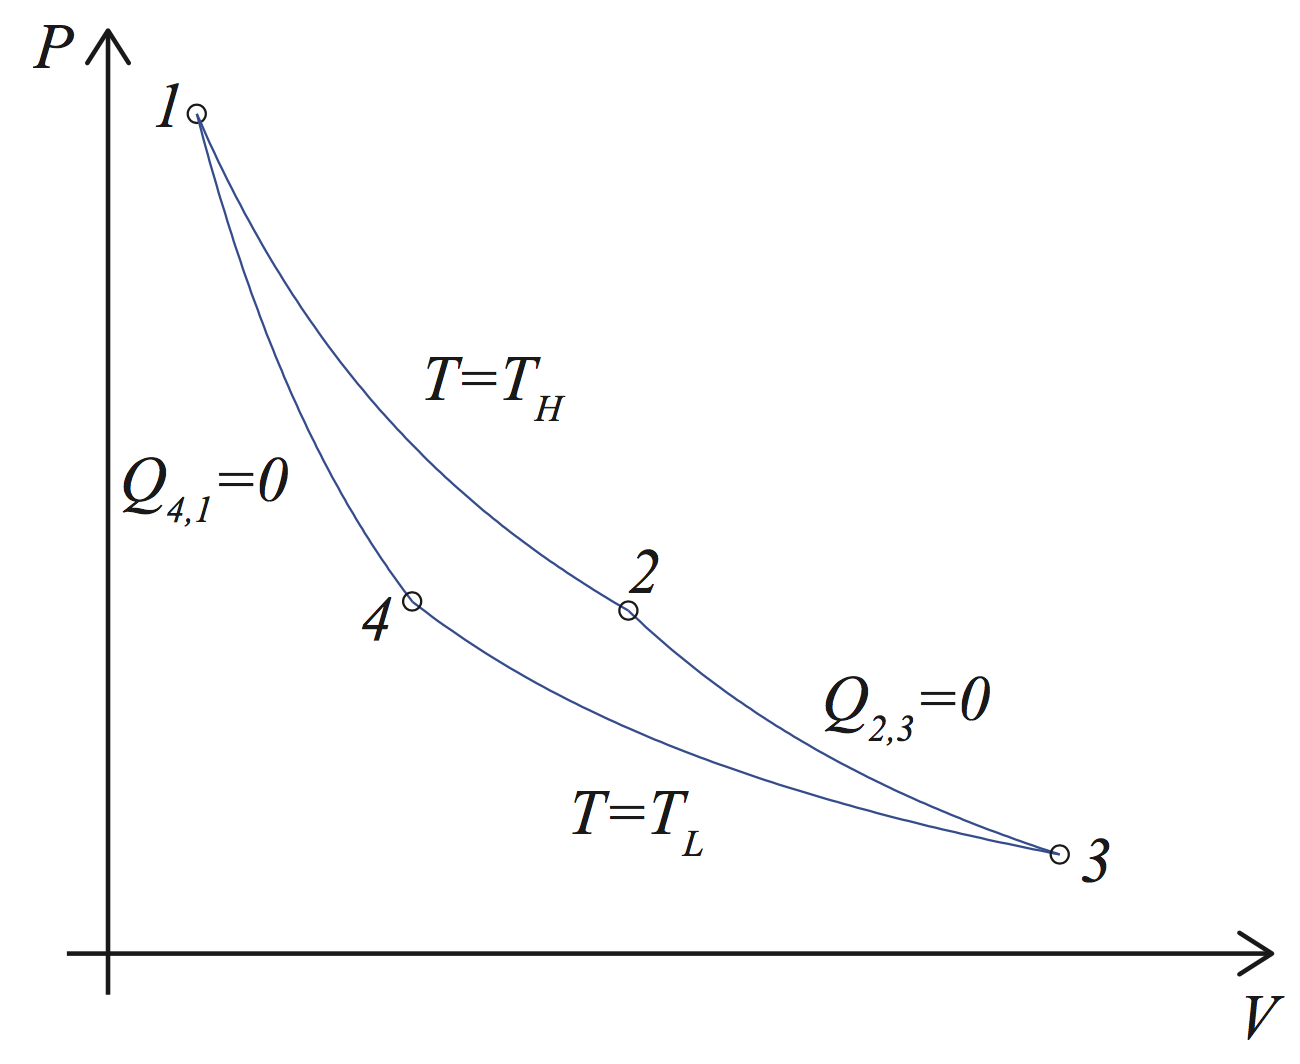
\includegraphics[width=0.30\textwidth]{carnot.png}
\end{figure}

\subsection{Refrigerators} A heat engine in reverse. Efficiency now called coefficient of performance $\text{COP}=\frac{Q_c}{W}=\frac{Q_c}{Q_h-Q_c} = \frac{1}{Q_h/Q_c -1}$. Some inequalities: $\frac{Q_h}{T_h} \geq \frac{Q_c}{T_c}$ which gives $\frac{Q_h}{Q_c} \geq \frac{T_h}{T_c}$. One can conclude $\text{COP} \leq \frac{1}{T_h/T_c -1} =\frac{T_c}{T_h - T_c}$.

\section{Free energy and Chemical thermodynamics}
Processes that are not cyclic. Interaction with environment s.t. $T$ and $P$ are constant, not $E$ and $V$.

\subsection{Free Energy as Available work}
Environment with constant $P$, related to \emph{enthalpy} is \textbf{Helmholtz free energy}: $F \equiv U - TS = U - T\Delta S$. Energy needed to create system, minus energy for from environment at temp $T$. 

Environment with constant $P$ and $T$, work needed to create/destroy is Gibbs free energy $G = U - TS + PV = H - TS$. The magician needs not the entire enthalpy, some comes for free as heat.

The four functions $U$, $H$, $F$ and $G$ are called \textbf{thermodynamic potentials}. Identities: $H$: $dH = dU + PdV + VdP = TdS + VdP + \mu dN$, $F$: $dF = dU - TdS - SdT = -SdT - PdV + \mu dN$, $S = -\left(\frac{\partial F}{\partial T} \right)_{V,N}$, $P = \left(\frac{\partial F}{\partial V} \right)_{T,N} $, $\mu = \left( \frac{\partial F}{\partial  N} \right)_{T,P} $. $G$: $dG = -SdT + VdP + \mu dN $, $S = - \left(\frac{\partial G}{\partial T} \right)_{P,N}$, $V = \left(\frac{\partial G}{\partial P} \right)_{T,N}$, $\mu = \left(\frac{\partial G}{\partial N} \right)_{T,P}$.

Example of \textbf{Maxwell relation}: $\left(\frac{\partial}{\partial V}\left(\frac{\partial U}{\partial S} \right)_{V,N} \right)_{S,N}$\\ $= \left(\frac{\partial}{\partial S}\left(\frac{\partial U}{\partial V} \right)_{S,N} \right)_{V,N}$ $\rightarrow \left(\frac{\partial T}{\partial V} \right)_S = - \left(\frac{\partial P}{\partial S} \right)_V$.

\subsection{Free Energy as a Force toward Equilibrium}
An increase in total entropy. Constant $N$, $U$, $V$: $S$ increase. Constant $N$, $T$, $V$: $F$ decrease. Constant $N$, $T$, $P$: $G$ decrease. Extensive properties: $V,N,S,U,H,F,G,m$. Intensive properties: $T,P,\mu, \rho$.

\subsection{Phase Transformations of Pure Substances}
The \textbf{Clausius-Clapyron relation}: $G_l = G_g$ at phase boundary, to remain $G_l = dG_g$. Thermodynamic identity for $G$:  $-S_ldT + V_ldP = -S_gdT + V_gdP$ gives $\frac{dP}{dT} = \frac{S_g-S_l}{V_g-V_l}$. Write $S_g-S_l = \frac{L}{T}$, where $L$ is latent heat, to get $\frac{dP}{dT} = \frac{L}{T\Delta V}$. Applies to the slope of any phase boundary line on a $PT$ diagram.

The \textbf{van der Waals equation} is $\left(P + \frac{aN^2}{V^2}\right)(V-Nb) = NkT$. Mod of ideal gas with molecular interaction.

\section{Boltzmann Statistics}

\subsection{The Boltzmann factor}
System in contact with reservoir and assume equal probability for all microstates. Boltzmann factor $=e^{-E(s)/kT}$\\ Partition function:  $Z = \sum_s e^{-E(s)/kT}$. Botlzmann/canonical distribution:  $\mathcal{P}(s) = \frac{1}{Z}e^{-E(s)/kT}$.

\subsection{Average Values}
$\bar{X} = \sum_s X(s) P(s)$. $\bar{E} = -\frac{1}{Z} \frac{\partial Z}{\partial \beta} = -\frac{\partial \ln Z}{\partial \beta}$. Example: Rotation of diatomic molecules (2 rot d.o.f.). Assuming low density. Allowed energies $E(j) = j(j +1)\epsilon$, $j=0,1,\dots$ with degeneracy $\Omega(j) ) 2j + 1$. Then $X_{rot} = \sum_{j=0}^\infty (2j+1) e^{-E(j)/kT}$. One can approximate with an integral if $kt >> \epsilon$: $Z_{rot} \approx \int_0^\infty (2j+1) e^{-E(k)/kT}dj = \frac{kT}{\epsilon} \rightarrow \bar{E} = kT$ in agreement with the equipartition theorem (identical atoms, divide by $2$). $C_V = \frac{\partial \bar{E}}{\partial T} = k$. At low $T$, $C_V \rightarrow 0$ according to third law. Agrees with exact $Z$. 

\subsection{The Equipartition Theorem}
Applies to systems with energy in the form of quadratic degrees of freedom: $E(q) = cq^2$ where $c$ is a constant and $q$ is a coordinate or momentum variable ($x$, $p_x$, $L_x$). Each $q$ corresponds to a separate, independent state. Pretend they're discretely spaced, separated by intervals $\Delta q$. $Z=\sum_q e^{-\beta cq^2} \approx \frac{1}{\Delta q} \int_{-\infty}^\infty e^{-\beta cq^2} dq$. Approximate to integral if $\Delta q$ is small. Bell curve. Calculate $\bar{E}=\frac{1}{2}kT$ from this to confirm equipartition theorem. Only true in high $T$ limit, or when spacing b/w energy levels i much less than $kT$.

\subsection{The Maxwell Speed Distribution}
From equipartition theorem, $v_{rms} = \sqrt{\frac{3kT}{m}}$. This is an average, we want a distributions for speed of molecules. $v$ can vary continuously $\rightarrow$ infinitely small probabilities. Use intervals, area under graph: $\mathcal{P}(v_1\dots v_2)=\int_{v_1}^{v_2}\mathcal{D}(v)dv$, where $\mathcal{P}(v) \propto e^{-mv^2/2kT}$ and $\mathcal{D}(v) \propto \mathcal{P}(v) \times \Omega(v)$, where $\Omega (v)$ is no of vectors $\vec{v}$ corresponding to $v$ ($\propto 4\pi v^2$). Must be set of vectors on surface of sphere with $\text{Area} = 4\pi v^2$. Then $\mathcal{D}(s) = C \cdot 4\pi v^2 e^{-mv^2/2kT}$. Find $C$ by normalising, with substitute $x=\sqrt{m/2kT}$, $1 = 4\pi C \left(\frac{2kT}{m} \right)^{3/2} \int_0^\infty x^2e^{-x^2}dx \rightarrow C = (m/2\pi kT)^{3/2}$. Final result: $\mathcal{D}(v) = \left( \frac{m}{2\pi kT}\right)^{3/2} 4\pi v^2 e^{-mv^2/2kT}$, note that $\bar{v}=\sqrt{\frac{8kT}{\pi m}}$.

\subsection{Partition Functions and Free Energy}
System at fixed $U$ in contact with reservoir at $T$. $Z(T)$ analogous to $\Omega(T)$. $F=U-TS=-kT\ln Z$, tends to decrease. $S=-\left(\frac{\partial F}{\partial T}\right)_{V,N}$, $P=-\left(\frac{\partial F}{\partial V}\right)_{T,N}$, $\mu=+\left(\frac{\partial F}{\partial N}\right)_{T,V}$.

\subsection{Partition Functions for Composite Systems}
\textbf{Two particles}: $ Z_{tot} = \sum_s e^{-\beta[E_1(s) + E_2(s)]} = \sum_s e^{-\beta E_1(s)} e^{-\beta E_2(s)}$. Distinguishable $ Z_{tot} = \sum_{s_1} \sum_{s_2} e^{-\beta E_1(s_1)} e^{-\beta E_2(s_2)} = Z_1 Z_2$. Indistinguishable  $Z_{tot} = \frac{1}{2} Z_1 Z_2$. \textbf{$N$ particles}: Distinguishable $ Z_{tot} = Z_1 Z_2 Z_3 \dots Z_N $. Indistinguishable $ Z_{tot} = \frac{1}{Z!}Z_1^N $. Assumes low density, i.e. no interaction between particles.

\subsection{Ideal gas revisited}
Boltzmann factors $ e^{-E(s)/kT} = e^{-E_{tr}(s)/kT} e^{-E_{int}(s)/kT} $, additionally $ Z_1 = Z_{tr} Z_{int} $. Translational first: Standing wave patterns are limited to $ \lambda_n = \frac{2L}{n} $, using de Broglie ($p=h/\lambda$), $ p_n = \frac{h}{\lambda_n}=\frac{hn}{2L} $. Energy-momentum relation ($E=p^2/2m$), $ E_n = \frac{p_n^2}{2m}=\frac{h^2n^2}{8mL^2}$. $ Z_{\text{1D}} = \sum_n e^{-E_n/kT} = \sum_n e^{-h^2n^2/8mL^2 kT}$. Integral approx $ Z_{\text{1D}} = \int_0^{\infty} e^{-h^2n^2/8mL^2 kT} dn = \frac{\sqrt{\pi}}{2} \sqrt{\frac{8mL^2kT}{h^2}} = \sqrt{\frac{2\pi mkT}{h^2}}L \equiv \frac{L}{\ell_Q}$. In 3D: $ E_{tr} = \frac{p_x^2}{2m} + \frac{p_y^2}{2m} + \frac{p_z^2}{2m}$ and $ Z_{tr} = \frac{L_x}{\ell_Q}\frac{L_y}{\ell_Q}\frac{L_z}{\ell_Q} = \frac{V}{v_Q} $. Partition function for one particle: $ Z_1 = \frac{V}{v_Q}Z_{int}$ and for $N$: $ Z = \frac{1}{N!} \left(\frac{V Z_{int}}{v_Q} \right)^N $.

\section{Quantum Statistics}

\subsection{The Gibbs Factor}
$\text{Gibbs factor} = e^{-[E(s)-\mu N(s)]/kT}$. $\mathcal{P}(s) = \frac{1}{\mathcal{Z}}e^{-[E(s)-\mu N(s)]/kT}$. The grand partition function $\mathcal{Z} = \sum_s e^{-[E(s)-\mu N(s)]/kT}$.

\subsection{Bosons and Fermions}
Particles with integer spin are bosons, while particles with half-integer spin are fermions. Two identical fermions cannot occupy the same space (\textbf{Pauli exclusion principle}). If $Z_1 >> N$ chance of two particles in same state is negligible. For ideal gas $Z_1 = \frac{V Z_{int}}{v_q} $.The quantum volume is $ v_Q = \ell_Q^3 = \left( \frac{h}{\sqrt{2\pi mkT}} \right)^3 $, a cube of the average de Broglie wavelength. Then: $ \frac{V}{N} >>v_q$. Distance b/w particles must be greater than de Broglie w.l.
\textbf{Fermi-Dirac}: $n$ can only be $0$ or $1$, so $\mathcal{Z} = 1 + e^{-(\epsilon-\mu)/kT}$. Occupancy: $ \bar{n} = \sum_n = n\mathcal{P}(n) = 0 \cdot \mathcal{P}(0) + 1 \cdot \mathcal{P}(1) = \frac{e^{-(\epsilon - \mu)/kT}}{1 + e^{-(\epsilon - \mu)/kT}} $. Simplification yields distribution $\bar{n}_{FD} = \frac{1}{e^{(\epsilon-\mu)/kT} + 1} $.
\textbf{Bose-Einstein}: $n$ can be any non-negative integer, so the grand partition function is $ \mathcal{Z} = 1 + e^{-(\epsilon-\mu)/kT} + e^{-2(\epsilon-\mu)/kT} + \dots = 1 + e^{-(\epsilon-\mu)/kT} + (e^{-(\epsilon-\mu)/kT})^2 + \dots = \frac{1}{1-e^{-(\epsilon-\mu)/kT}}$. $\mu$ must be less than $\epsilon$, the series must converge. Occupancy: $ \bar{n} = \sum_n n \mathcal{P}(n) = 0 \cdot \mathcal{P}(0) + 1 \cdot \mathcal{P}(1) + 2 \cdot \mathcal{P}(2) + \dots $, abbreviate $x \equiv (\epsilon-\mu)/kT$. Then $\bar{n} = \sum_n \frac{e^{-nx}}{\mathcal{Z}} = -\frac{1}{\mathcal{Z}} \sum_n \frac{\partial}{\partial x} e^{-nx} = -\frac{1}{\mathcal{Z}}\frac{\partial\mathcal{Z}}{\partial x}$. Distribution: $ \bar{n}_{BE} = -(1-e^{-x})\frac{\partial}{\partial x}(1-e^{-x}) = (1-e^{-x})(1-e^{-x})^{-2}(e^{-x}) = \frac{1}{e^{(\epsilon-\mu)/kT-1}} $.
\textbf{Boltzmann/Classical} Prob for single particle in state $s$ is $\mathcal{P}(s) = \frac{1}{Z_1}e^{\epsilon/kT}$, average number in \emph{this} state is $\bar{n}_{B} = N\mathcal{P}(s) = \frac{N}{Z_1}e^{\epsilon/kT}$. Chemical potential is $\mu = -kT\ln(Z_1/N)$, which gives average occupancy $\bar{n}_B = e^{\mu/kT}e^{-\epsilon/kT}=e^{-(\epsilon-\mu)/kT}$. In this limit quantum effects are negligible. 

\subsection{Degenerate Fermi Gases}
At $t=0$ Fermi-Dirac becomes step function. All states $\epsilon_s < \mu$ are occupied and v.v. $\mu$ is the \textbf{Fermi energy}: $ \epsilon_{F} \equiv \mu(T=0)$. A free electron in a box have allowed wavelengths $ \lambda_n = \frac{2L}{n}, \quad p_n = \frac{h}{\lambda_n} = \frac{hn}{2L} $, in 3D $ p_x = \frac{hn_x}{2L}$ etc. which yields allowed energies $ \epsilon = \frac{\mid {\vec{p} \mid }^2}{2m} = \frac{h^2}{8mL}(n_x^2 + n_y^2 + n_z^2) $. $\epsilon_F$ is the energy of a state that sits just on the surface of an eight-sphere in "$n$-space", so $ \epsilon_F = \frac{h^2n^2_{max}}{8mL^2} $. Because fermions have two spin orientations, the number of occupied states is twice the volume of an eight-sphere $ N = 2 \times (\text{volume of eigth-sphere}) = 2 \cdot \frac{1}{8} \cdot \frac{4}{3} \pi n^3_{max} = \frac{\pi n^2_{max}}{3} $. Combining gives the Fermi energy $ \epsilon_F = \frac{h^2}{8m} \left( \frac{3N}{\pi V} \right)^{2/3} $.

The number of states in $n$-space with magnitude $n$ between $n$ and $n+dn$ is $ D(n)dn = 2 \cdot \frac{1}{8} \cdot 4 \pi n^2 dn = \pi n^2 dn $. No of states: $ N = \sum_{n_x,n_y,n_z} 2\bar{n}(\epsilon(n_x,n_y,n_z), \mu, T)$\\$= \int_0^{\infty} \bar{n}(\epsilon(n), \mu, T)D(n)dn $. Avg energy:\\ $ \bar{E} = \sum_{n_x,n_y,n_z} 2\epsilon(n_x,n_y,n_z)\bar{n}(\epsilon(n_x,n_y,n_z), \mu, T)$\\$= \int_0^{\infty}\epsilon(n)\bar{n}(\epsilon(n), \mu, T)D(n)dn $. Substitute: $ d\epsilon(n) = \frac{d\epsilon}{dn}dn $. Which gives $ N = \int_0^{\infty} \bar{n}(\epsilon(n), \mu, T)D(n(\epsilon))\frac{1}{d\epsilon / dn} d\epsilon $ and \\$ \bar{E} = \int_0^{\infty}\epsilon(n)\bar{n}(\epsilon(n), \mu, T)D(n(\epsilon))\frac{1}{d\epsilon / dn} d\epsilon$. See that $ D(n)dn = D(\epsilon)d\epsilon $. Apply relation $ \epsilon(n) = \frac{\hbar}{2m}\left( \frac{\pi}{L} \right)^2 n^2 = an^2 $ $\rightarrow$ $ n = \sqrt{\frac{\epsilon}{a}} \quad \text{and} \quad \frac{d\epsilon}{dn} = 2an $. Then: $ D(\epsilon) = D(n)\frac{1}{d\epsilon / dn} = \pi n^2 \frac{1}{2an} = \frac{\pi}{2a}n = \frac{\pi}{2a} \sqrt{\frac{\epsilon}{a}}
        = \frac{\pi}{2a^{3/2}}\epsilon^{1/2} = \frac{\pi(8m)^{3/2}}{2h^3}V\sqrt{\epsilon} = \frac{3N}{2\epsilon_F^{3/2}}\sqrt{\epsilon} $.

\subsection{Blackbody Radiation}
QHO allowed energies: $E_n = 0, hf, 2hf, \dots$. Partition function: $Z = 1 \ e^{-\beta hf} + e^{-2\beta hf} + \dots = \frac{1}{1-e^{-\beta hf}}$. Average energy: $\bar{E} = -\frac{1}{Z}\frac{\partial Z}{\partial \beta} = \frac{hf}{e^{hf/kT}-1}$. Average number of units of energy is $\bar{n}_{Pl} = \frac{1}{e^{hf/kT}-1}$.

\subsection{Bose-Einstein Condensation}
Energy of atoms in box: $\epsilon_0 = \frac{3h^2}{8mL^2}$. Atoms in this state (B-E):\\ $N_0 = \frac{1}{e^{(\epsilon_0-\mu)(kt} - 1}$. Taylor series gives $ \frac{kT}{\epsilon_0 - \mu}$. Total number of atoms approximated by integral $N = \int_0^{\infty} g(\epsilon) \frac{1}{e^{(\epsilon - \mu)/kT} - 1} d\epsilon$. Density of states: $g(\epsilon) = \frac{2}{\sqrt{\pi}}\left( \frac{2\pi m}{h^2} \right)^{3/2} V\sqrt{\epsilon}$. Guess $\mu = 0$, switch $x= \epsilon/kT$. $N = \frac{2}{\sqrt{\pi}}\left( \frac{2\pi m}{h^2} \right)^{3/2} V \int_0^\infty \frac{\sqrt{\epsilon}d\epsilon}{e^{\epsilon/kT}-1} = \frac{2}{\sqrt{\pi}}\left( \frac{2\pi m kT}{h^2} \right)^{3/2} V \int_0^\infty \frac{\sqrt{x}dx}{e^x - 1}$. The integral is $2.315$. Wrong result. $N_{excited} = 2.612 \left(\frac{2\pi m kT}{h^2} \right)^{3/2} V = \left(\frac{T}{T_c} \right)^{3/2}N$ when $T < T_c$. Rest is in ground state, $N_0 = N-N_{excited} = \left[1- \left(\frac{T}{T_c} \right)^{3/2} \right]N$. Abrupt accumulation of atoms in ground state at temperatures below $T_c$ is called \textbf{Bose-Einstein condensation}.

\section*{Scripts}
$E = \sum_{i=1}^N aS_i$
\lstinputlisting[firstline=4, lastline=10, frame=single]{../programs/spinsystem.py}
Random matrix of $-1$ and $1$.
\lstinputlisting[firstline=3, lastline=12, frame=single]{../programs/randomstate.py}

\end{document} 